
%\documentclass[options]{class}
\documentclass[10pt,journal]{IEEEtran}

%Paquete de Idioma
\usepackage[spanish]{babel}
\usepackage{graphicx}

%Codificación Alfabeto
\usepackage[utf8]{inputenc}
\usepackage{amsmath}
\usepackage{amsfonts}
\usepackage{amssymb}
%\usepackage{amstext} 

%Codificación de Fuente
\usepackage[T1]{fontenc}

%Estilo de Página Numeración superior
%\pagestyle{headings}

%Hiperlinks \href{url}{text}
\usepackage[pdftex]{hyperref}

\usepackage{graphicx}

\begin{document}

%Titulo
\title{Naturaleza y propagación de la luz}

%Autor
\author{Fernando Dalai Aguilar Sánchez \\ Laboratorio de óptica, ESFM-IPN, Ciudad de México, México \\Febrero 28 de 2023}


\maketitle{}  

%Resumen
\begin{abstract}
La primera sesión práctica llevada a cabo en el laboratorio de óptica tuvo como objetivo estudiar la naturaleza y propagación de la luz, mediante la realización de dos experimentos de gran relevancia en el campo de la óptica.
En el primer experimento, se midió el índice de reflexión y refracción de dos materiales diferentes.
En el segundo experimento, se realizó la observación de la sombra generada por un objeto en relación a una fuente de luz. 
\end{abstract}  

\section{Introducción}
A la luz también se le puede denominar como radiación electromagnética visible; esto
es, es aquella radiación que produce sensación visual en el ojo humano y corresponde a
una porción muy angosta del espectro electromagnético, mejor conocida como la región
visible del espectro.

La energía electromagnética en una longitud de onda λ particular (en el vacío) tiene una
frecuencia f asociada y una energía de fotón E. Por tanto, el espectro electromagnético
puede ser expresado igualmente en cualquiera de esos términos. Se relacionan en las
siguientes ecuaciones: 
\begin{align}
c = \lambda f \\
E = \dfrac{h c}{\lambda}
\end{align}
donde $c = 299{,}792{,}458$ es la velocidad de la luz y h es la constante de Planck. 

Por lo tanto, las ondas electromagnéticas de alta frecuencia tienen una longitud de onda
corta y mucha energía mientras que las ondas de baja frecuencia tienen grandes
longitudes de onda y poca energía.

Por encima de la frecuencia de las radiaciones infrarrojas se encuentra lo que
comúnmente llamamos luz. Es un tipo especial de radiación electromagnética que tiene
una longitud de onda en el intervalo de 0,38 a 0,73 $\mu$m. Hasta hace relativamente poco
tiempo la unidad usual para expresar las longitudes de onda era el Angstrom, Ǻ. Sin
embargo, debido a que se ha fomentado el uso del Sistema Internacional de Unidades SI
para expresar las unidades de las magnitudes físicas, las unidades que se emplean hoy
en día son principalmente el micrómetro ($\mu$m) o el nanómetro (nm).

La sombra, penumbra y región de máxima iluminación son conceptos fundamentales en el estudio de la óptica y la iluminación.
La sombra es el área que queda completamente oscura debido a la ausencia de luz, y se produce cuando un objeto bloquea por completo la fuente de luz que incide sobre él. La penumbra, por su parte, es el área donde la luz es bloqueada parcialmente por el objeto, lo que resulta en una disminución de la intensidad luminosa. Finalmente, la región de máxima iluminación es el área donde la luz incide directamente sin obstrucciones y con mayor intensidad.

\section{Metodología}


\subsection{Experimento 1. Reflexión y refracción de la luz.}
Para el primer experimento se empleo una mesa circular donde se coloco al centro de esta un recipiente con dos diferentes fluido, el experimento consistia en disparar un laser al recipiente y observar la reflexión y refracción sobre un espejo plano.


.
\begin{figure}[!ht]
\begin {center}
\includegraphics[width=0.4\textwidth]{8.jpg}
\caption{Experimento 1.}
\end {center}
\end{figure}

Para el primer fluido se obtuvieron los siguientes datos:
\begin{center}
\begin{tabular}{|c|c|c|c|}
\hline
N & $\theta$i & $\theta$r & $\theta$t \\
\hline
1 & 10 & 17.1 & 7\\
\hline
2 & 20 & 37.3 & 12.9\\
\hline
3 & 30 & 57.3 & 19.4\\
\hline
4 & 40 & 77.5 & 25.5\\
\hline
5 & 50 & 97.5 & 31\\
\hline
6 & 60 & 118.1 & 36\\
\hline
7 & 70 & 137.9 & 40\\
\hline
8 & 80 & 158.3 & 42.4\\
\hline
\end{tabular}
\end{center}

Al representarlos gráficamente, obtenemos:

\begin{figure}[!ht]
\begin {center}
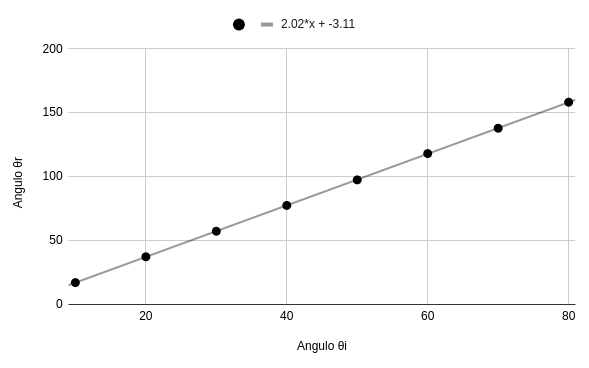
\includegraphics[width=0.4\textwidth]{1.png}
\caption{Grafica $\theta$r vs $\theta$i}
\end {center}
\end{figure}

\begin{figure}[!ht]
\begin {center}
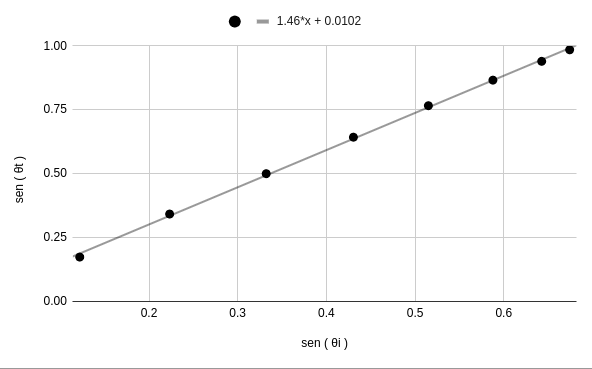
\includegraphics[width=0.4\textwidth]{2.png}
\caption{Grafica sen($\theta$t) vs sen($\theta$i)}
\end {center}
\end{figure}


Para el segundo fluido se obtuvieron los seguientes datos:

\begin{center}
\begin{tabular}{|c|c|c|c|}
\hline
N & $\theta$i & $\theta$r & $\theta$t \\
\hline
1 & 10 & 18 & 6.6\\
\hline
2 & 20 & 37.8 & 13.2\\
\hline
3 & 30 & 57.8 & 19.8\\
\hline
4 & 40 & 78 & 25.7 \\
\hline
5 & 50 & 98.1 & 31.2 \\
\hline
6 & 60 & 118.4 & 35.9 \\
\hline
7 & 70 & 138.5 & 39.9\\
\hline
8 & 80 & 158.5 & 42.7 \\
\hline
\end{tabular}
\end{center}


Al representarlos gráficamente, obtenemos:

\begin{figure}[!ht]
\begin {center}
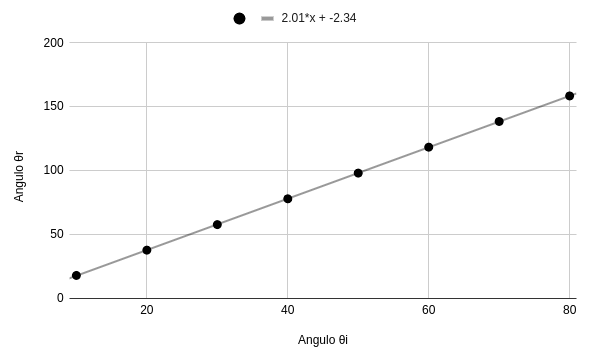
\includegraphics[width=0.4\textwidth]{3.png}
\caption{Grafica $\theta$r vs $\theta$i}
\end {center}
\end{figure}

\begin{figure}[!ht]
\begin {center}
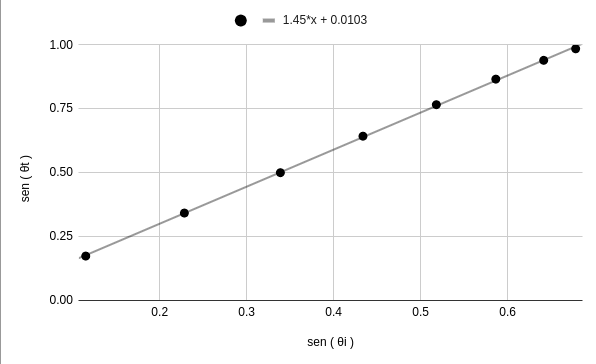
\includegraphics[width=0.4\textwidth]{4.png}
\caption{Grafica sen($\theta$t) vs sen($\theta$i)}
\end {center}
\end{figure}

.

\subsection{Experimento 2. Sombra, penumbra y región de máxima iluminación.}
Para el segundo experimento se utilizó un objeto opaco en forma de cruz al cual se le colocaba enfrente una fuente de luz puntual para poder observar la sombra que este generaba sobre una hoja de papel dependiendo de la abertura de la fuente.



\begin{figure}[!ht]
\begin {center}
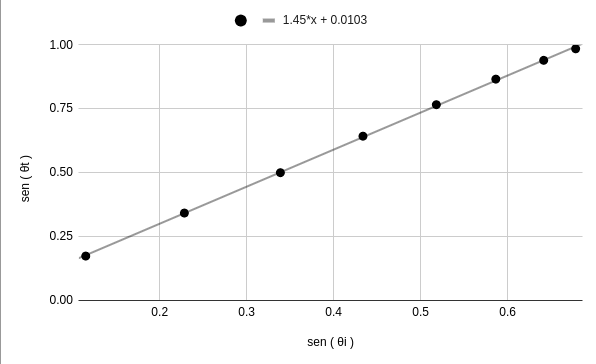
\includegraphics[width=0.4\textwidth]{4.jpg}
\caption{Experimento 2.}
\end {center}
\end{figure}


\begin{figure}[!ht]
  \centering
  \rotatebox{270}{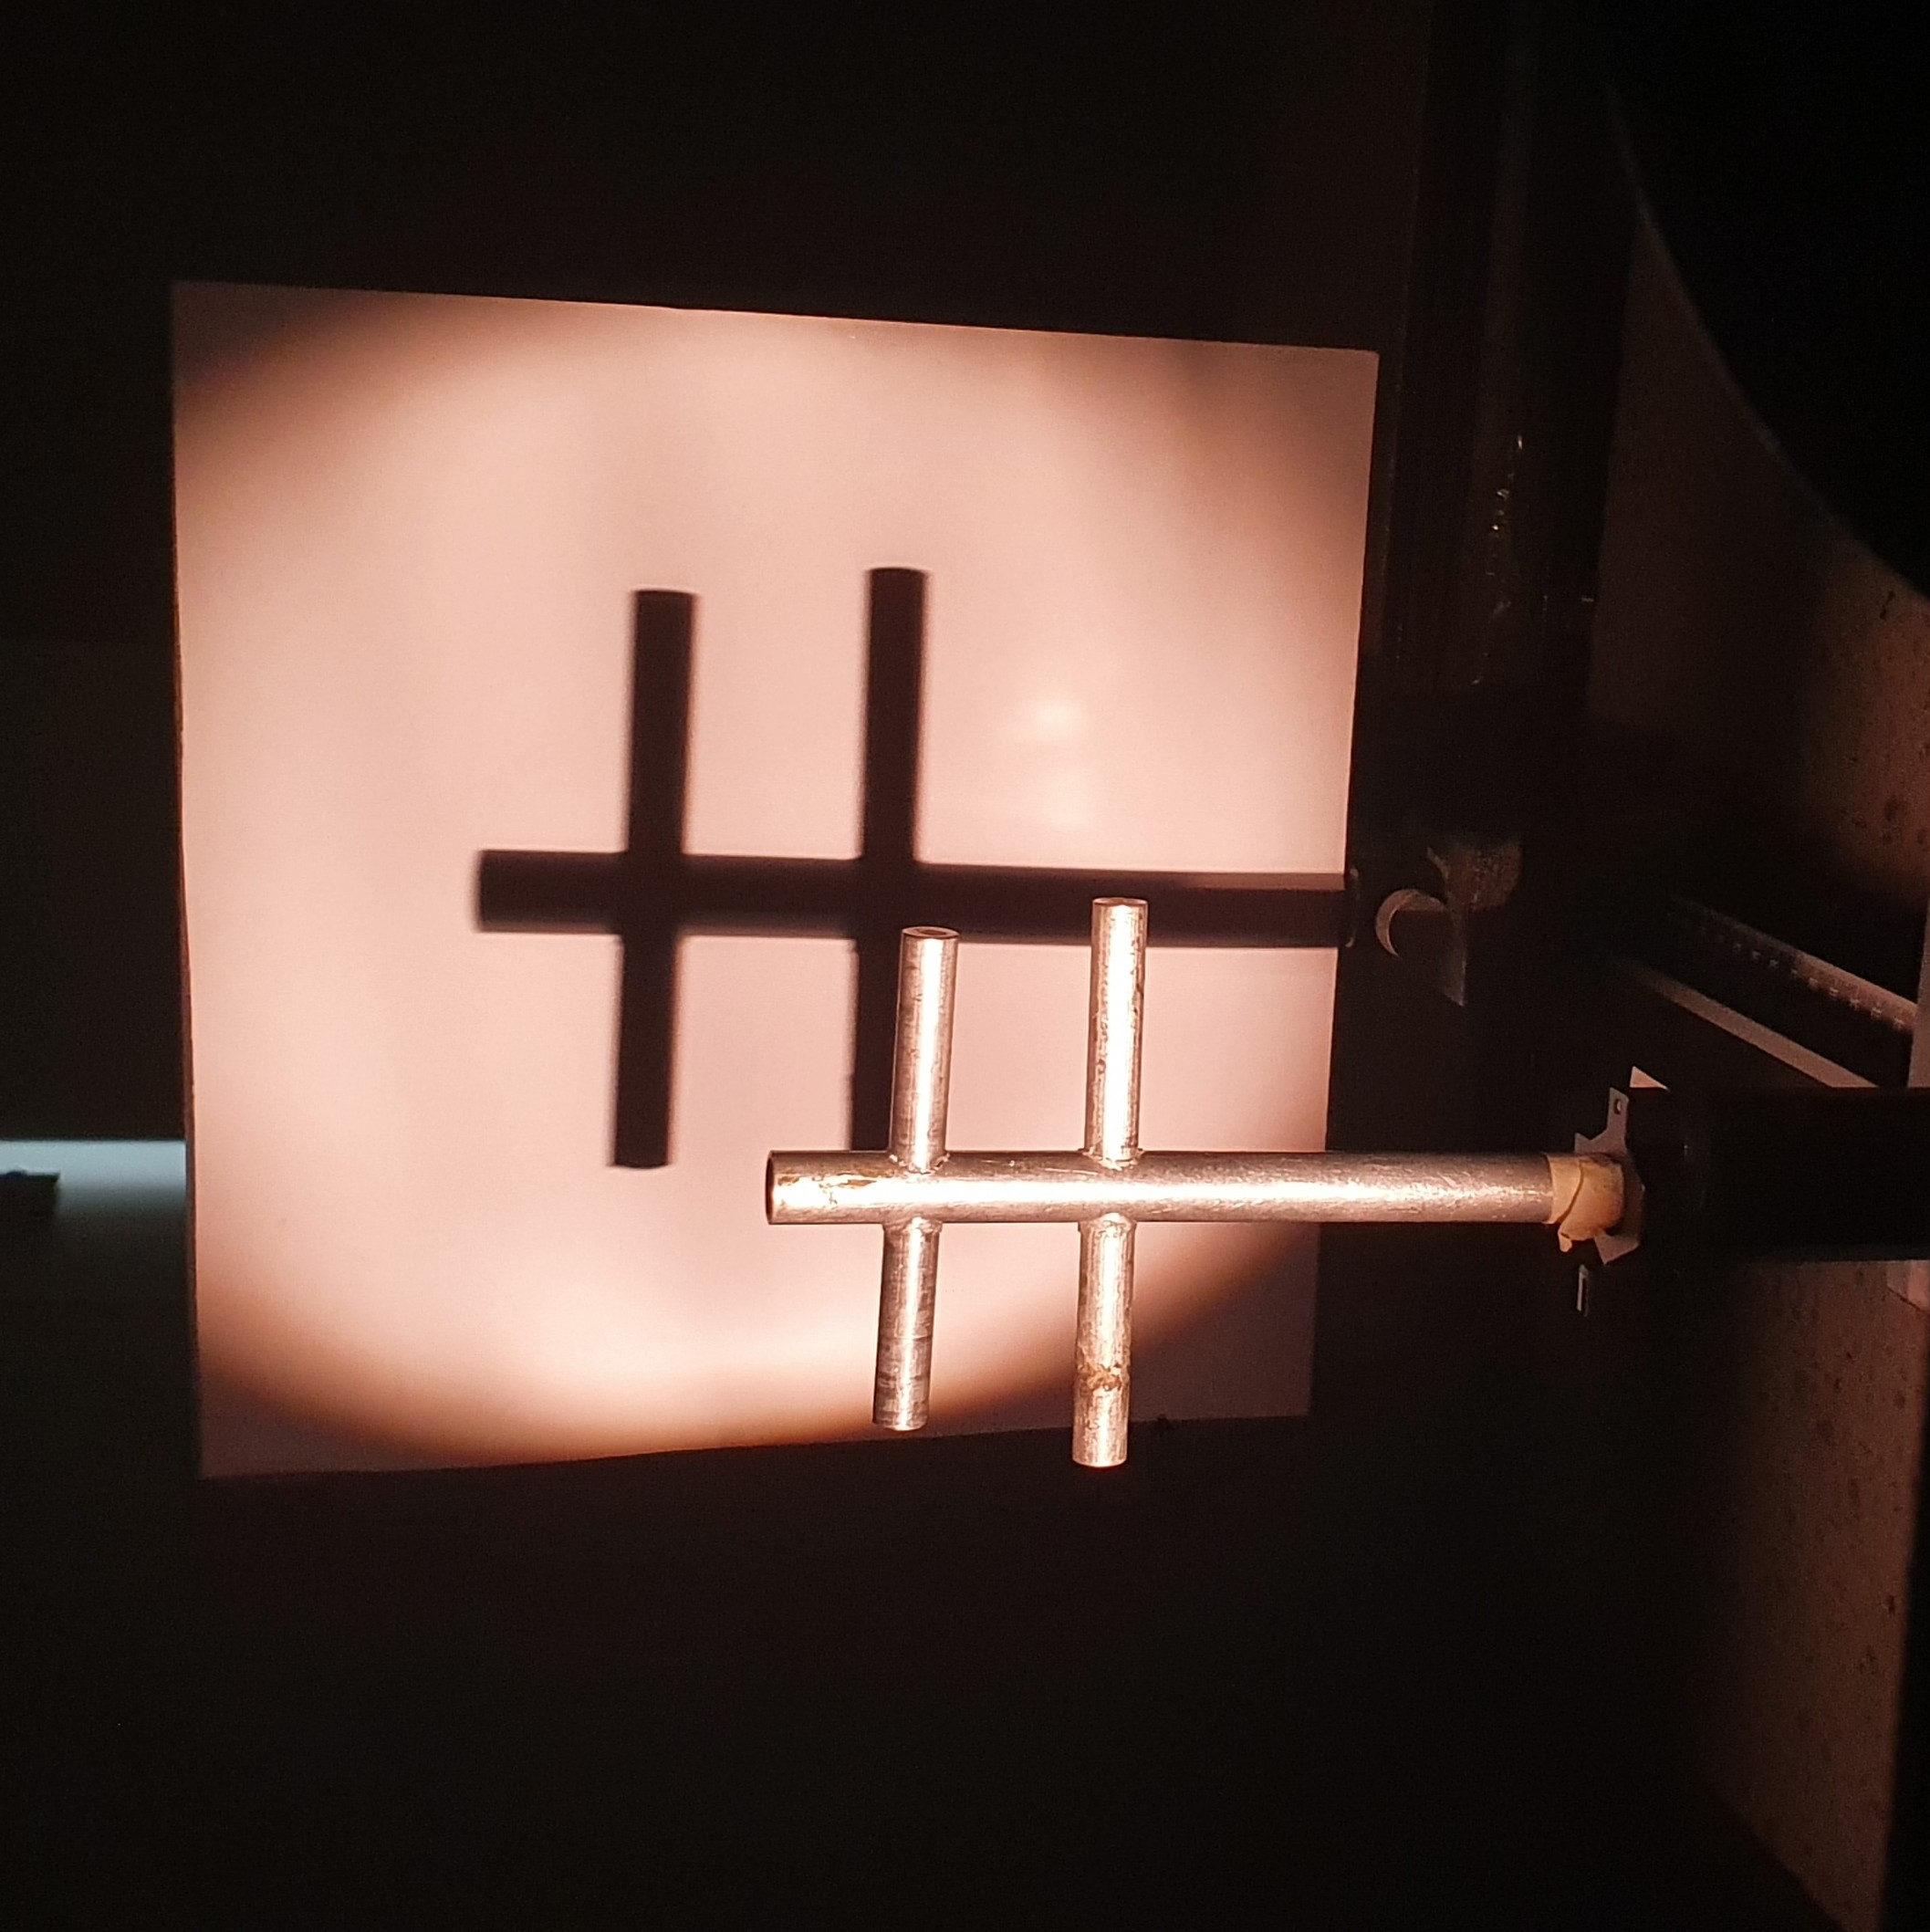
\includegraphics[width=0.4\textwidth]{s1.jpg}}
  \caption{Sombra generada en el experimento 2}
  \label{fig:myimage}
\end{figure}

\section{Discusión y conclusiones}

\subsection{Reflexión y refracción de la luz.}
\item 

De acuerdo a los datos obtenidos en el experimento de reflexion, tanto para el primer fluido como para el segundo, nos damos cuenta que se sigue la siguiente relacion $\theta_r \approx 2\theta_i$ lo cual es lo que se esperaria teoricamente. 

Para las mediciones de la refraccion, si observamos las funciones de ajuste obtenidas y empleamos la ley de Snell:
\begin{align*}
    n_1\sin\theta_1 &= n_2\sin\theta_2 \\
\end{align*}

podemos obtener los indices de refraccion de ambos fluidos. Para el primero tenemos:
\begin{align*}
\quad \frac{\sin\theta_1}{\sin\theta_2} &= 1.43
\end{align*}

por lo que  se podria tratar se de fluoruro de calcio. Para el segundo fluido tenemos:
\begin{align*}
\quad \frac{\sin\theta_1}{\sin\theta_2} &= 1.45
\end{align*}
por lo que se podemos concluir que se trata de aceite vegetal.
\item 


\subsection{Sombra, penumbra y región de máxima iluminación.}
Para llevar a cabo este experimento, hemos podido observar que existen diversos factores que influyen en la sombra que se proyecta dependiendo del haz de luz que emana de nuestra fuente. Específicamente, hemos notado que el tamaño de la sombra y su nitidez pueden variar de acuerdo con la apertura del haz de luz.

Es importante destacar que, en nuestra observación, se pudo percibir que a medida que se aumentaba la abertura del haz de luz, la sombra se volvía más nítida y clara. 

Estas observaciones son de gran relevancia para el estudio de la óptica y su aplicación en diferentes campos, como la fotografía, la iluminación y la proyección de imágenes
\item 






\section{Bibliografía}


Resnick, Halliday y Krane, (2002). Física. VOl I. México. Editorial Cecsa.


Serway, R.A., Jewett, J.W. (2009). "Física: Para ciencia e ingeniería con Física Moderna", 7 Edicion. Vol.2 México. Cengage.


W. Sears, MW Zemansky, HD Young y R. A. Freedman: "Física universitaria", 12 Edición. VOl 2. Addison-Wesley-Longman/Pearson Education.



\end{document}